\subsection{Semiconductors} \label{chap3}

(Source \cite[Elementary Solid State Physics Chapter 6]{elementary_SSP})

\subsubsection*{Question 1}
The carrier distribution function in CB für an intrinsic semiconductor
is given as the product:

$$g_e(E) f(E)$$

with

$$g_e(E) = \frac{1}{2\pi^2} \left( \frac{2m_e^*}{\hbar} \right)^\frac{3}{2} (E-E_C)^\frac{1}{2}$$

$$f(E) = \frac{1}{e^{(E-E_F)/k_BT}+1}  \approx e^{-\frac{E-E_F}{k_BT}}$$

So for the maximum 

$$\frac{d}{dE} \left(\frac{1}{2\pi^2} \left( \frac{2m_e^*}{\hbar} \right)^\frac{3}{2} (E-E_C)^\frac{1}{2} e^{-\frac{E-E_F}{k_BT}} \right) = 0$$

By dividing through the constant factors:

$$\frac{d}{dE} \left( (E-E_C)^\frac{1}{2} e^{-\frac{E}{k_BT}} \right) = 0$$

$$\frac{1}{2} (E-E_C)^{-\frac{1}{2}} e^{-\frac{E}{k_BT}} + \frac{-1}{k_BT} (E-E_C)^\frac{1}{2} e^{-\frac{E}{k_BT}} = 0$$

And finaly

$$E = E_C + \frac{k_BT}{2}$$


\subsubsection*{Question 2}

For the effective density of states in theh conducition beand 
the following relation is known:

$$ N_c = 2 \left( \frac{m_e^*k_BT}{2\pi\hbar^2}\right)^{\frac{3}{2}}$$

Which lead to the following result
$$ N_c = 2.415 \cdot 10^{24} \frac{1}{m^3}$$

In the same manner also the density of states in the valence band can be
calculatetd.

$$ N_v = 2 \left( \frac{m_h^*k_BT}{2\pi\hbar^2}\right)^{\frac{3}{2}}$$
$$ N_v = 1.796 \cdot 10^{25} \frac{1}{m^3}$$

In an intrinsic semiconductor the concentration of the holes and the 
electron are equal and this concentration is named as
intrinsic carrier's concentration. 

Which is knwon to be:
$$n_i = p_i = 2 \left( \frac{k_BT}{2\pi\hbar^2} \right)^{\frac{3}{2}}
  (m_e^*m_h^*)^{\frac{3}{4}} e^{-\frac{E_g}{2k_BT}}$$
$$n_i = p_i = 0.959 \cdot 10^3 \frac{1}{m^3}$$

For the intrinsic Fermi can be calculatetd as 

$$E_{Fi} = \frac{E_g}{2} + \frac{3}{4} k_B T \ln\left( \frac{m_h^*}{m_e^*} \right)$$

$$E_{Fi} = 1.326 eV$$


\subsubsection*{Question 3}

If the given semiconductor CdS was doped p-type with a
concentration of $10^{15}$ acceptor impurities the following
about the concentration and holes at $T=0\degree K$ can be said.

At this point the thermal energy becomes too small to cause electron exication, which means that all electrons fall from
the conducition Band into the donor level. Also the conductivity
goes to zero. This process is called freeze out. 
So for the concentration of electron and holes at $T=0 \degree K$

The concentration of the elctrons:

$n(T=0 \degree K) = 0$

As the semiconductor is doped with holes the concentration of the
holes is the same as it was initaly.

$p(T=0 \degree K) = 10^{15}cm^{-3}$


\subsubsection*{Question 4}

As the concentration of acceptor impurities is much higher then
the holes concentration of the intrinsic semiconductor 
$(10^{15} \frac{1}{cm^3} \gg p_i)$

The concentration of the holes in the semiconductor is equal to concentration
of the impurities.

$$p = 10^{15} \frac{1}{cm^3} = 10^{18} \frac{1}{m^3}$$

As the square of the intrinsic concentrationn$n_i$ is equal to the product
of the sum of the concentration of the holes and the concentration of the
electrons.

$$np = n_i^2$$

$$n = \frac{n_i^2}{p} = \frac{(0.959 \cdot 10^3 \frac{1}{m^3})^2}{10^{18} \frac{1}{m^3}} = 9.197 \cdot 10^{-13} \frac{1}{m^3}$$

As for calculating $(E_F-E_{Fi})$ the temperature dependence of the
concentration on electrons and holes can be used:

$$n = n_i e^{\frac{E_F-E_{Fi}}{k_BT}}  \qquad p = n_i e^{-\frac{E_F-E_{Fi}}{k_BT}}$$

Which leads to:

$$(E_F-E_{Fi}) = \ln\left( \frac{n}{n_i} \right) \cdot k_BT$$

$$(E_F-E_{Fi}) = -0.896 eV $$

\subsubsection*{Question 5}

As the potential for Hole is given as:

\begin{equation}
  V(r) = -\frac{e^2}{4\pi \epsilon_r \epsilon_0 r}
\end{equation}

By using the Bohr model, the beinding energy can be found, which
corresponds to the ground state of the acceptor and calculatetd.
With using $\epsilon_r = 8.9$ and $m_h = 0.80\,m_0$


$$
E_a = \frac{1}{\epsilon_r^2} \left(\frac{m_h}{m_0}\right) \underbrace{\left[\frac{e^4m_0}{2(4\pi\epsilon_h\hbar)^2}\right]}_{13.6eV}
$$

$$E_a =  0.14eV$$

\autoref{fig:acceptorLevel} shows the acceptor level inside the energy gap.

\begin{figure}[H]
  \centering
  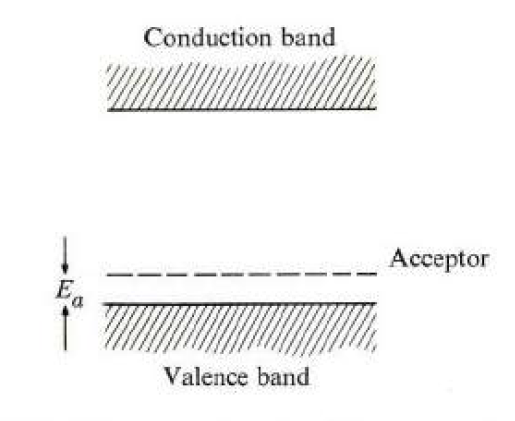
\includegraphics[width=0.35\linewidth]{Graphics/Chapter3/acceptorLevel.png}
  \caption{The acceptor level in a semiconductor \cite[Elementary Solid State Physics p. 268]{elementary_SSP} }
  \label{fig:acceptorLevel}
\end{figure}

\subsubsection*{Compensated semiconductor Question 6}

Compensated semiconductor are those in which donors and acceptors are related in such a way that their opposing electrical effects are partially cancelled
In the compensated semiconductor there are additional sources of current carriers and therefore
$$
n - p = \Delta n \neq 0.
$$
Fermi energy value $\epsilon_F$ in the doped semiconductor will change relative to $\epsilon_{F(i)}$ values for an intrinsic semiconductor. From here we can write the equation
$$
n = n_i exp\bigg[+\frac{\epsilon_F - \epsilon_{F(i)}}{k_B T}\bigg] \ \mathrm{and} \
p = p_i exp\bigg[-\frac{\epsilon_F - \epsilon_{F(i)}}{k_B T}\bigg]
$$
Taking both of those formulas we get this relation
\begin{equation}
\frac{\Delta n}{n_i} = 2\sinh{\bigg[\frac{\epsilon_F - \epsilon_{F(i)}}{k_B T}\bigg]}
\end{equation}
In donor semiconductors $\Delta n > 0$ so Fermi energy $\epsilon_F > \epsilon_{F(i)}$ \\
In acceptor semiconductors $\Delta n < 0$ so Fermi energy $\epsilon_F < \epsilon_{F(i)}$

\subsubsection*{Intrinsic resistivity Question 7}
In order to determine resistivity of the intrinsic cadmium sulfide (CdS) at 300 K, proceed as follows. In an intrinsic semiconductor electron carrier concentration $n$ equals to hole concenctration $p$ and this both equals intrinsic carrier concetration $n_i$. That is
$$
n = p = n_i 
$$
The resistivity $\rho$ of the intrinsic semiconductor is given by
$$
\rho_{intrinsic} = \frac{1}{q(\mu_nn + \mu_pp)}
$$
where charge $q = 1.6 \times 10^{-19}\ \mathrm{C}$, electron mobility is $\mu_n$ and hole mobility is $\mu_p$.
\begin{equation}
CalculationS
\end{equation}

\subsubsection*{Direct and Indirect Band Gab Question 8}

In \autoref{fig:CDS-Band} the Band Gab structure $E(\vec{k})$ for CdS and ZnS as 
a model result is showed.

\begin{figure}[H]
  \centering
  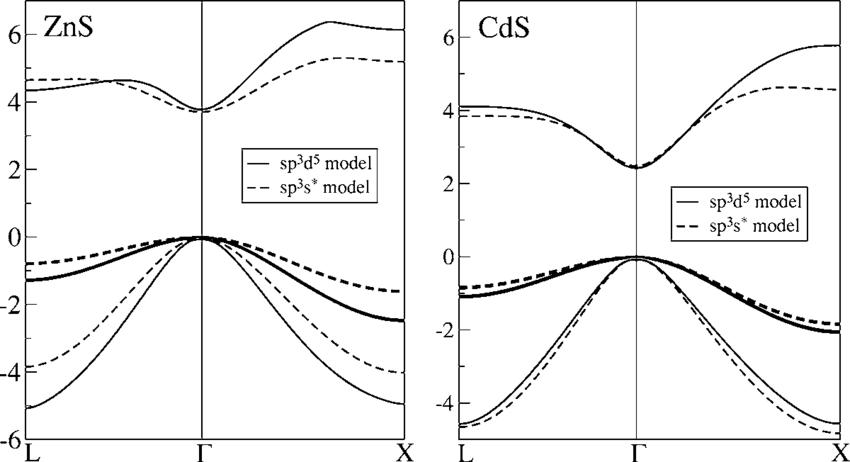
\includegraphics[width=0.7\linewidth]{Graphics/Chapter3/Bulk-band-structure-for-ZnS-and-CdS-along-the-L-111-and-the-X-100-directions-obtained.png}
  \caption{Bulk band structure for ZnS and CdS along the-L 111 and the-X 100 directions obtained with the sp 3 d 5 
  model solid line and the sp 3 s * model of Lippens \cite{band_gap_CdS}}
  \label{fig:CDS-Band}
\end{figure}

As the minimum of the conduction band as well as the maximum of the valence band are both 
at $\Gamma$ ($\vec{k}= 0)$. CdS can be identified as a semiconductor with
direct Band Gap.

As the Band Gap Energy is minimal at $k=0$, it will incease 
with $T$ due to the added kinetic energie to the electrons.

The Band Gap Energie can be easily measured by use of the fact
that below the $E_G$ no or only little absorbiton occurs.

By measuring the absorbiton coefficient $\alpha$ in a 
semiconductor as a function of $hv$ an egde will appear 
where $\alpha$ rapidly raises. At this energy the electron
can move to the conducition band and absorb the photon.
 

\subsubsection*{Free excition Question 9}

An exciton is a bound state of an electron and an electron hole which are attracted to each other by the electrostatic Coulomb force. It is an electrically neutral quasiparticle that exists in insulators, semiconductors and some liquids. The exciton is regarded as an elementary excitation of condensed matter that can transport energy without transporting net electric charge.

\subsubsection*{P-N junction Question 10}

A $P-N$ junction is the juxtaposition of a n-type and a p-type piece of semiconductor, taken originally from the same block of crystal. The difference between the densities of donors and acceptors $ND - NA$ undergoes a very sharp variation from a negative value in the $P$ region to a positive value in the N region. An abrupt junction is by definition a junction in which the doping type changes over a very small distance compared to the spatial extent of the depletion region
When the junction meets thermal equilibrium, the Fermi energy has a constant value throughout the whole device. The energies of conduction and valence bands are therefore shifted up or down, and exhibit a smooth variation across the depletion region. As a consequence, there is an electrostatic potential energy difference appearing between the $P$ and $N$ region, equal to $qV_d$.

\begin{figure}[H]
  \centering
  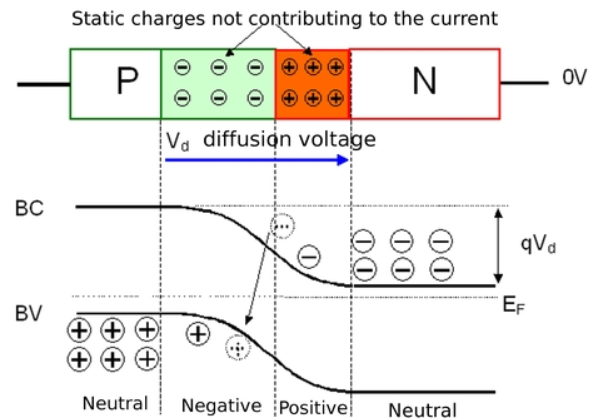
\includegraphics[width=0.35\linewidth]{Graphics/Chapter3/PNjunction.PNG}
  \caption{Energy diagram of a PN junction at thermal equilibrium\cite{PN}}
  \label{fig:PNjunction}
\end{figure}

For a p–n junction, letting  $C_A(x)$ and $C_D(x)$ be the concentrations of acceptor and donor atoms respectively, and letting  $N_0(x)$ and $P_0(x)$ be the equilibrium concentrations of electrons and holes respectively, yields, by Poisson's equation:v
$$
-\frac{d^2V}{dx^2} = \frac{\rho}{\epsilon} = \frac{q}{\epsilon}[(P_0 - N_0) + (C_D - C_A)]
$$
where V is the electric potential, $\rho$ is the charge density, $\epsilon$ is permittivity and $q$ is the magnitude of the electron charge. Letting $d_p$  be the width of the depletion region within the p-side, and letting $d_n$ be the width of the depletion region within the n-side, it must be that
$$
d_pC_A = d_nC_D
$$
because the total charge on either side of the depletion region must cancel out. Therefore, letting $D$ and $\Delta V$ represent the entire depletion region and the potential difference across it,
$$
\Delta V = \int \int \frac{q}{\epsilon}[(P_0 - N_0) + (C_D - C_A)] dxdx = \frac{C_AC_D}{C_A + C_D} \frac{q}{2\epsilon} (d_p + d_n)^2
$$
where $P_0 = N_0 = 0$ because we are in the depletion region. And thus, letting = $d$ be the total width of the depletion region, we get
$$
d = \sqrt{\frac{2 \epsilon}{q} \frac{C_A + C_D}{C_AC_D} \Delta V}
$$
$\Delta V$ can be written as $\Delta V_0 + \Delta V_{ext}$ , where we have broken up the voltage difference into the equilibrium plus external components. The equilibrium potential results from diffusion forces, and thus we can calculate $V$  by implementing the Einstein relation and assuming the semiconductor is nondegenerate
$$
V = \frac{k_B T}{e} \ln\bigg(\frac{n_n}{n_p}\bigg)
$$